\section{Component controls and representation sensitivity}\label{sec:components}
\subsection{Frozen component-removal experiment}
A follow-up experiment isolates the explicit mask-input channel, nearest-support-distance input, and coverage-weighted pooling of MIRA-CSI. Four controlled configurations retain the same 20-channel architecture, 40,871 nominal trainable parameters, initialization at each seed, source partitions, augmentation draws, optimizer, checkpoint rule and clean-source temperature calibration. The reference retains all three components. The other configurations respectively zero the mask-input channel, zero the distance-input channel, or replace coverage weighting with uniform temporal averaging. Zeroing an input retains its nominal parameters but removes its data-dependent gradient. In particular, removing the explicit mask input does not remove all missingness information: distance and coverage weighting remain available.

Two standard residual 1D CNNs provide separate architecture-and-capacity comparators, with and without source loss augmentation. Each has three residual blocks of 64/128/128 channels, convolutions of lengths 7/5/3, GroupNorm and GELU, followed by eight-bin temporal averaging and a seven-class head; each has 511,111 parameters. Their architecture is a reference design rather than a new MIRA component. Architecture and parameter count change together, so these models are not component-level ablations and do not isolate a capacity effect. The residual models use the same source-only optimizer, epoch-selection and calibration settings as the compact networks. CUDA-safe explicit temporal-bin means implement the declared pooling operation.

The six configurations, three outer folds and five training seeds produce 90 source-fitted models. All checkpoints and calibration parameters were frozen and hashed before this follow-up evaluation. Each model is tested on complete input and the full five-mask grid of random/contiguous 50\% loss under all three repairs: 31 conditions on both familiar and held sets. This retains 5,580 metric rows and 1,640,520 probability vectors. These are repeated views of the same recordings, not additional participants. Independent arithmetic reconstruction reproduced every metric row, with maximum absolute difference $4.44\times10^{-16}$. A separate CPU audit loaded every frozen checkpoint and reproduced 15,120 source-validation prediction views without a classification-label mismatch; the maximum CPU/T4 logit difference was $6.20\times10^{-6}$.

The follow-up is exploratory: its design responds to results already observed on this dataset. Freezing the new fits prevents target-dependent selection within this execution, but does not make the historical target data an untouched external confirmation set. For a corrupted condition, held predictions are first pooled across the three folds for each training/mask-seed cell. Scores are then averaged across five masks within each training seed, and the mean and sample SD are reported across the five training seeds. This differs from the initial paired-seed summary in Table~\ref{tab:expanded}.

\begin{table*}[t]
\centering\begin{minipage}{\textwidth}
\refstepcounter{table}\label{tab:components}
{\fontsize{9.3}{12}\selectfont\textbf{Table~\thetable.} Frozen follow-up held accuracy (\%). Corrupted conditions average all five mask realizations within each training seed; cells show mean $\pm$ sample SD across five training seeds after pooling the three held sets. R50/B50 use linear repair. All four MIRA configurations have 40,871 nominal trainable parameters; both residual controls have 511,111.\par}
\vspace{5pt}\begingroup\sffamily\fontsize{9.2}{12}\selectfont
\setlength{\tabcolsep}{6pt}\renewcommand{\arraystretch}{1.5}
\begin{tabularx}{\linewidth}{>{\raggedright\arraybackslash}p{.34\linewidth}*{3}{>{\centering\arraybackslash}X}}
\rowcolor{foresthead}\multicolumn{1}{l}{\textcolor{white}{\bfseries Configuration}} & \multicolumn{1}{c}{\textcolor{white}{\bfseries Complete}} & \multicolumn{1}{c}{\textcolor{white}{\bfseries R50}} & \multicolumn{1}{c}{\textcolor{white}{\bfseries B50}}\\
\rowcolor{mintfill}MIRA full reference & $23.73\pm2.26$ & $22.68\pm2.03$ & $22.56\pm1.28$\\
\rowcolor{referencefill}Zero explicit mask input & $23.41\pm1.03$ & $23.22\pm1.23$ & $21.90\pm0.53$\\
\rowcolor{mintfill}Zero distance input & $24.03\pm1.87$ & $22.85\pm1.87$ & $22.77\pm1.02$\\
\rowcolor{referencefill}Uniform temporal pooling & $24.17\pm2.54$ & $23.22\pm1.86$ & $21.30\pm1.57$\\
\rowcolor{lossfill}Residual CNN, clean training & $33.83\pm0.82$ & $33.33\pm0.87$ & $26.72\pm0.67$\\
\rowcolor{shiftfill}Residual CNN, augmented & $30.25\pm1.65$ & $30.09\pm1.70$ & $25.72\pm1.35$\\
\end{tabularx}\endgroup\end{minipage}\end{table*}

\begin{figure*}[t]
\centering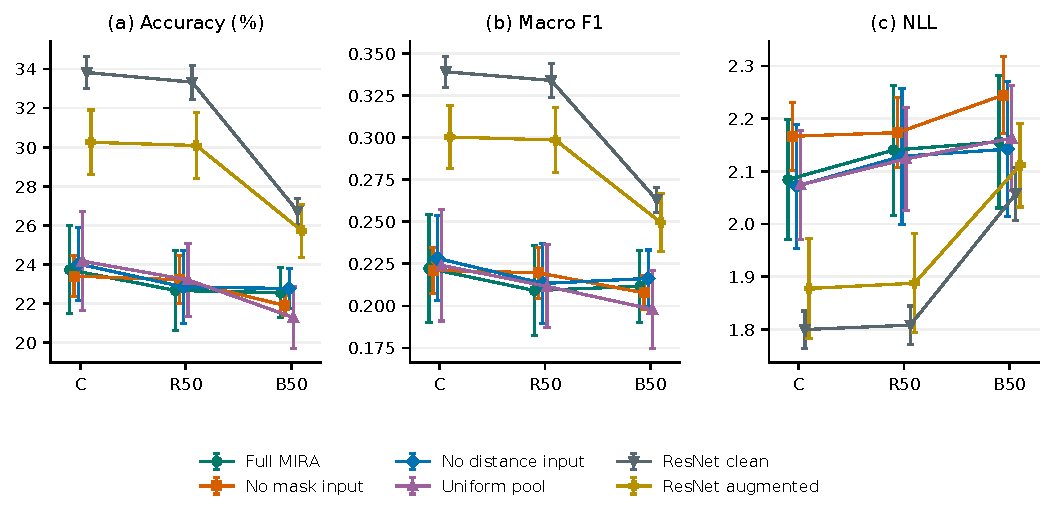
\includegraphics[width=\textwidth]{component_model_comparison.pdf}
\caption{Frozen follow-up comparison of accuracy, macro F1 and source-temperature-calibrated NLL. C is complete input; R50/B50 are random/contiguous 50\% loss with linear repair. Metrics pool 1,260 held files within each training/mask cell, then average masks within training seed. Points show means and bars sample SD across five training seeds on fixed recordings and partitions; they are not confidence intervals for new environments. Higher accuracy/F1 and lower NLL are preferred.}
\label{fig:componentmodels}
\end{figure*}

The larger residual clean-training control reaches 33.83\% held accuracy on complete input and 26.72\% under block loss (Table~\ref{tab:components}, Figure~\ref{fig:componentmodels}); its augmented counterpart reaches 30.25\% and 25.72\%. The residual architectures improve these particular compact-network results, but changing architecture and capacity together does not identify the cause of that difference or establish a generally optimal model. The full MIRA reference reproduces its original clean accuracy. Its block value here averages the full mask grid and therefore differs from the earlier five paired-mask summary. SD across these five mask-averaged seed summaries is not the same quantity as SD across the original five diagonal training/mask pairs. For conditionally independent, identically distributed mask draws within a fixed fit, averaging five masks reduces that fit's mask-variance component by a factor of five; this is not a rule for the total variability across trained models.

For component contrasts, 10,000 paired participant-cluster bootstrap draws sample ten participants with replacement within each fixed environment and retain their complete seed/mask grid. The full model minus each of the three removal controls under linear B50 defines one three-comparison macro-F1 family. Table~\ref{tab:componentcontrasts} reports ordinary 95\% percentile ranges and Bonferroni-adjusted 98.333\% marginal percentile ranges for that family. These approximate conditional sensitivity ranges remain exploratory, depend on within-environment participant exchangeability and fixed fitted models, and do not cover new rooms, retraining or all secondary outcomes. The resampling unit is the participant rather than an individual mask view.

\begin{table*}[t]
\centering\begin{minipage}{\textwidth}
\refstepcounter{table}\label{tab:componentcontrasts}
{\fontsize{9.3}{12}\selectfont\textbf{Table~\thetable.} Component contrasts under contiguous 50\% loss with linear repair. Differences are full MIRA minus the named control in pooled macro F1. The second column adds sample SD of paired, mask-averaged differences across five training seeds; the final column counts positive seed differences. Percentile ranges share identical participant draws, condition on the fixed fitted models, and address only the three contrasts shown.\par}
\vspace{5pt}\begingroup\sffamily\fontsize{9.1}{12}\selectfont
\setlength{\tabcolsep}{5pt}\renewcommand{\arraystretch}{1.5}
\begin{tabularx}{\linewidth}{>{\raggedright\arraybackslash}p{.27\linewidth}>{\centering\arraybackslash}p{.17\linewidth}*{2}{>{\centering\arraybackslash}X}>{\centering\arraybackslash}p{.10\linewidth}}
\rowcolor{purplehead}\multicolumn{1}{l}{\textcolor{white}{\bfseries Control}} & \multicolumn{1}{c}{\textcolor{white}{\bfseries $\Delta$ F1 $\pm$ SD}} & \multicolumn{1}{c}{\textcolor{white}{\bfseries Conditional 95\%}} & \multicolumn{1}{c}{\textcolor{white}{\bfseries Adjusted 98.333\%}} & \multicolumn{1}{c}{\textcolor{white}{\bfseries Positive}}\\
\rowcolor{lavenderfill}Zero explicit mask input & $+0.0039\pm0.0126$ & $[-0.0074,0.0155]$ & $[-0.0096,0.0180]$ & $3/5$\\
\rowcolor{lavenderlight}Zero distance input & $-0.0047\pm0.0117$ & $[-0.0080,-0.0015]$ & $[-0.0086,-0.0007]$ & $2/5$\\
\rowcolor{lavenderfill}Uniform temporal pooling & $+0.0137\pm0.0190$ & $[0.0001,0.0275]$ & $[-0.0023,0.0302]$ & $4/5$\\
\end{tabularx}\endgroup\end{minipage}\end{table*}

The explicit mask-input contrast is inconclusive in this condition. Omitting the distance input gives a small higher mean macro F1 than the full reference, including under the declared conditional three-contrast adjustment; however, the paired difference changes direction across training seeds (Table~\ref{tab:componentcontrasts}). It is not a stable advantage across every initialization. Coverage weighting has a positive unadjusted range, but its adjusted range includes zero (Figure~\ref{fig:componentfamily}). Thus the experiment does not support presenting all three MIRA components as individually beneficial. These condition-specific findings neither prove that a component has no value elsewhere nor validate the full architecture as superior to the reference transform. Different complete-input scores after channel removal are also compatible with retraining under a different parameterization: even a constant clean mask channel can change convolutional activations and the optimization trajectory, including padding-boundary effects. No physical mechanism is identified by that score difference alone.

\begin{figure*}[t]
\centering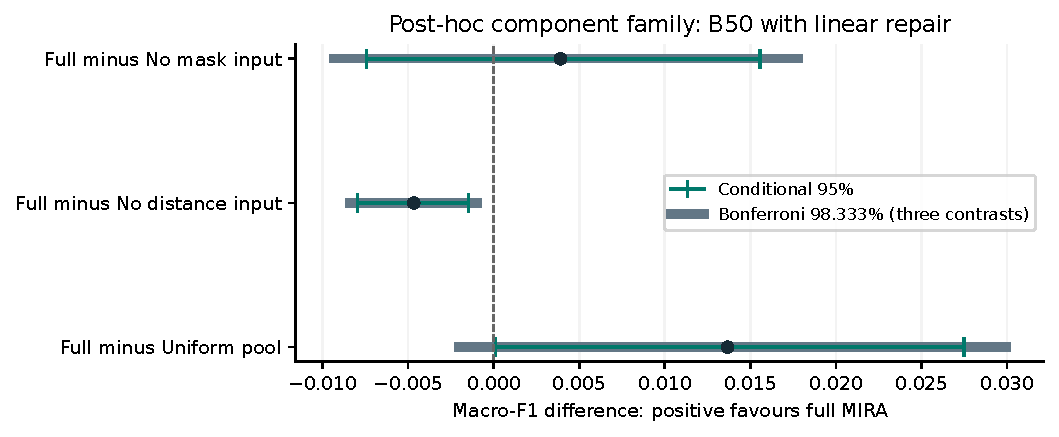
\includegraphics[width=\textwidth]{component_family_intervals.pdf}
\caption{Paired component differences under linear B50. Thin green segments with terminal ticks mark unadjusted 95\% participant-bootstrap percentile ranges; thick gray segments mark 98.333\% ranges adjusted for the three displayed contrasts. Each point is full MIRA minus a removal control, so positive values favour the full model. All ranges use the same 10,000 participant draws within the three fixed environment/cohort strata. This exploratory post-hoc analysis does not measure uncertainty over new environments or model retraining.}
\label{fig:componentfamily}
\end{figure*}


\subsection{Source-selected representation of the reference transform}
A separate clean-input sensitivity study strengthens the known MiniRocket comparator without attributing that algorithm to MIRA-CSI. Before fitting, five candidate input representations were fixed: the original bands, one scalar z-score per recording, a temporal z-score per band, source-training per-band 0.1/99.9-percentile winsorization, and log-mean-power bands. The last candidate averages scaled squared amplitudes before applying $10\log_{10}$ and retains the same 500-position resampling. It uses relative scaled power, not calibrated dBm. Source-only inspection motivated this numerical sensitivity check; changing the transform is not evidence of an architectural contribution.

Within each outer fold, representation selection uses only that fold's source-validation macro F1 at seed 20261026. Validation scores are never pooled across outer folds for selection, because another fold can contain the current target environment. The selected representation is then held fixed across all five seeds. E1 selects per-band temporal standardization; E2 and E3 select scalar recording standardization. MiniRocket remains the official 9,996-feature multivariate transform, with the same source-only feature scaling, ridge coefficient and temperature-fitting rule. All 30 reference/selected fits were sealed before any new held scoring; six seed-one fits were reused and 24 additional fits were trained.

\begin{table*}[t]
\centering\begin{minipage}{\textwidth}
\refstepcounter{table}\label{tab:representation}
{\fontsize{9.3}{12}\selectfont\textbf{Table~\thetable.} Clean-input MiniRocket representation sensitivity. Means $\pm$ sample SD across five seeds; metrics pool 1,260 held files per seed. The selected representation is chosen independently from each outer fold's source validation. This is a reference-transform improvement, not a new MIRA model.\par}
\vspace{5pt}\begingroup\sffamily\fontsize{9.1}{12}\selectfont
\setlength{\tabcolsep}{5pt}\renewcommand{\arraystretch}{1.5}
\begin{tabularx}{\linewidth}{>{\raggedright\arraybackslash}p{.25\linewidth}*{4}{>{\centering\arraybackslash}X}}
\rowcolor{navy}\multicolumn{1}{l}{\textcolor{white}{\bfseries Input representation}} & \multicolumn{1}{c}{\textcolor{white}{\bfseries Accuracy (\%)}} & \multicolumn{1}{c}{\textcolor{white}{\bfseries Macro F1}} & \multicolumn{1}{c}{\textcolor{white}{\bfseries NLL}} & \multicolumn{1}{c}{\textcolor{white}{\bfseries Brier}}\\
\rowcolor{lossfill}Original & $53.08\pm0.33$ & $0.531\pm0.003$ & $1.395\pm0.049$ & $0.639\pm0.008$\\
\rowcolor{shiftfill}Source-selected & $57.44\pm1.04$ & $0.574\pm0.009$ & $1.259\pm0.040$ & $0.586\pm0.013$\\
\end{tabularx}\endgroup\end{minipage}\end{table*}

The pooled accuracy difference is 4.37 percentage points (Table~\ref{tab:representation}). Per-environment mean accuracy changes from 57.24\% to 66.43\% in E1, 50.67\% to 50.43\% in E2, and 51.33\% to 55.48\% in E3. The gain is therefore not shared by every environment. Independent checks reconstructed scores from 12,600 saved held probability vectors and verified all 30 checkpoint hashes without repeating target inference. Recording standardization in this stage uses complete recordings; this clean-only experiment establishes neither missing-input robustness nor an information-safe standardization procedure under hidden-value loss. No inference about a new MIRA mechanism follows from the MiniRocket improvement.

The selected pipeline's seed SD is 1.04 percentage points, compared with 0.33 for the original representation. The representation choice is fixed from one source-validation seed; its stability across alternative selection seeds has not been measured. Furthermore, the CNNs were not subjected to the same five-candidate input-selection procedure. This sensitivity result therefore compares two declared MiniRocket pipelines and does not isolate an architectural cause for their differences from the neural models.
